\documentclass{article}
\usepackage{amsmath}
\usepackage{amssymb}
\usepackage[a4paper, top=25mm, bottom=25mm, left=25mm, right=25mm]{geometry}
\usepackage{pgfplots}
\usepackage{mathtools}
\usepgfplotslibrary{fillbetween}
\usepackage{cancel}
\pgfplotsset{compat=1.18}

\begin{document}
\pagestyle{empty}
\large

\begin{center}
2022-2023 Fall \\MAT123-02,05 Final\\(11/01/2023)
\end{center}

\noindent 1. The radius $R$ of a spherical ball is measured as $14$ in.

\hfill

\noindent (a) Use differentials to estimate the maximum propagated error in computing the volume $V$ if $R$ is measured with a maximum error of $1/8$ inches.

\hfill

\noindent (b) With what accuracy must the radius $R$ be measured to guarantee and error of at most $2$ in$^3$ in the calculated volume?

\hfill

\noindent 2. Evaluate the following integrals.

\hfill

\noindent (a) $\displaystyle\int\frac{dx}{\sqrt x\,\left(\sqrt x+2\right)}$

\hfill

\hfill

\noindent (b) $\xcancel{\displaystyle\int\frac{\sin x}{x^2+1}\,dx}$

\hfill

\hfill

\noindent (c) $\displaystyle\int\frac{dx}{\sqrt{3-x^2}}$

\hfill

\hfill

\noindent (d) $\displaystyle\int\frac{dx}{2+\cos x}$

\hfill

\noindent 3. Use the Shell Method and then the Washer Method to set up an integral (but do not evaluate) the volume of the solid generated by revolving the region $R$ about the $y$-axis, where $R$ is bounded by the curve $y=x^2$ and the line $y=-x+1$.

\hfill

\noindent 4. Find the area of the surface obtained by rotating the arc of the curve $\displaystyle y=\frac{x^3}6+\frac1{2x}$ on the interval $[1/2,1]$ about the $x$-axis.

\hfill

\noindent 5. Using the Integral Test, determine whether the series

\hfill

\noindent $\displaystyle\sum_{n=1}^\infty\frac2{3n+5}$

\hfill

\noindent converges or diverges.

\hfill

\noindent 6. Find the Maclaurin series for $\displaystyle f(x)=\frac1{x^2-5x+6}$.

\newpage

\begin{center}
2022-2023 Final (11/01/2023) Solutions\\
(Last update: 8/18/25 (18th of August) 1:51 AM)
\end{center}

\noindent 1.

\hfill

\noindent (a) The volume of a sphere with radius $r$ is

\[V=\frac43\pi r^3\]

\hfill

\noindent The differential of $V$ is

\[dV=4\pi r^2\,dr\]

\hfill

\noindent The maximum error is known to be $1/8$ inches. So, $|dr|\leq1/8$. The maximum propagated error is then

\[dV=4\pi\cdot14^2\cdot\dfrac18=\boxed{98\pi\:\text{in}^3.}\]

\hfill

\noindent (b) $|dV|=2$ at most. Solve the differential form for $dr$.

\[dr=\frac{dV}{4\pi r^2}=\frac{2}{4\pi\cdot 14^2}=\boxed{\frac1{392\pi}\:\text{inches}}\]

\hfill

\noindent 2.

\hfill

\noindent (a) Let $x=u^2$, then $u=\sqrt x$ and $dx=2u\,du$.

\begin{align*}\int\frac{dx}{\sqrt x\,\left(\sqrt x+2\right)}&=\int\frac{2u}{u(u+2)}\,du=2\int\frac{du}{u+2}=2\ln|u+2|+c\\\\&=\boxed{2\ln\left|\sqrt x+2\right|+c,\: c\in\mathbb{R}}\end{align*}

\hfill

\noindent (b) This question is beyond the scope of the curriculum, and students are not expected to solve it using the knowledge they have acquired in this course.

\hfill

\noindent (c) Let $x=\sqrt3\sin u$ for $-\dfrac\pi2<u<\dfrac\pi2$, then $dx=\sqrt3\cos u\,du$.

\begin{align*}\int\frac{dx}{\sqrt{3-x^2}}&=\int\frac{\sqrt3\cos u}{\sqrt{3-3\sin^2u}}\,du=\int\frac{\cos u}{\sqrt{\cos^2u}}\,du=\int\frac{\cos u}{|\cos u|}\,du\\\\&=\int\frac{\cos u}{\cos u}\,du\quad\left[\cos u>0\right]\\\\&=\int du=u+c\end{align*}

\hfill

\noindent If $x=\sqrt3\sin u$, then $\sin u=\dfrac x{\sqrt3}\implies u=\arcsin\left(\dfrac x{\sqrt3}\right)$. The answer is then

\hfill

\[\boxed{\arcsin\left(\frac x{\sqrt3}\right)+c,\quad c\in\mathbb{R}}\]

\hfill

\noindent (d) We may utilize the tangent half-angle substitution, which is sometimes called the Weierstrass substitution. Let $\displaystyle t = \tan\left(\frac x2\right)$. Then

\begin{equation*}
\sin x={\frac{2t}{1+t^{2}}},\quad\cos x={\frac{1-t^{2}}{1+t^{2}}},\quad dx={\frac2{1+t^{2}}}\,dt
\end{equation*}

\hfill

\noindent Rewrite the integral.

\[\int\frac{dx}{2+\cos x}=\int\frac{\dfrac2{1+t^2}}{2+\dfrac{1-t^2}{1+t^2}}\,dt=\int\frac{2}{3+t^2}\,dt=\int\frac{2}{3\left(1+\dfrac{t^2}3\right)}\,dt=\frac23\int\frac1{1+\left(\dfrac t{\sqrt3}\right)^2}\,dt\]

\hfill

\noindent Let $u=\dfrac t{\sqrt3}$, then $\sqrt3\,du=dt$.

\begin{align*}\frac23\int\frac{dt}{1+\left(\dfrac t{\sqrt3}\right)^2}&=\frac{2\sqrt3}3\int\frac{du}{1+u^2}=\frac{2\sqrt3}3\arctan u+c=\frac{2\sqrt3}3\arctan\frac t{\sqrt3}+c\\&=\boxed{\frac{2\sqrt3}3\arctan\left(\frac1{\sqrt3}\tan\left(\frac x2\right)\right)+c,\quad c\in\mathbb{R}}\end{align*}

\hfill

\noindent 3.
\begin{center}
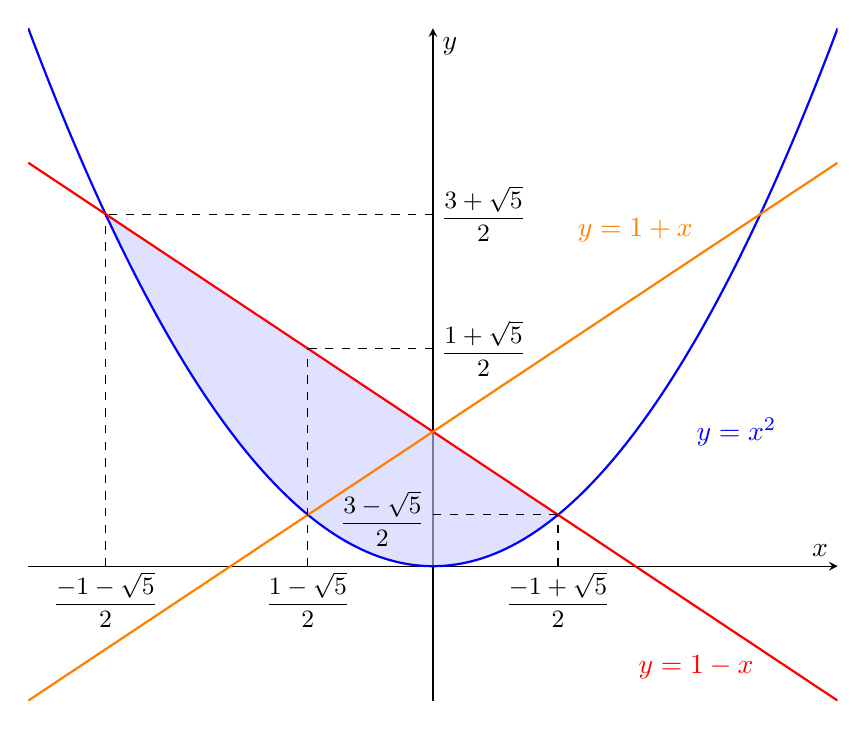
\begin{tikzpicture}
  \begin{axis}[
      axis lines=center,
      xlabel={$x$},
      ylabel={$y$},
      ytick=\empty, xtick=\empty,
      xmin=-2, xmax=2,
      ymin=-1, ymax=4,
      samples=250,
      clip=true,
      scale=1.5,
      domain=-2:2,
    ]

    \addplot [thick, blue, name path=A] {x^2};
    \addplot [thick, red, name path=B] {-x+1};
    \addplot [thick, orange] {x+1};
    \addplot [blue!20, fill opacity=0.6] fill between[of=A and B, soft clip={domain=-1.618:0.618}];
    
    \node at (-1.618,-0.25) {\small $\displaystyle\frac{-1-\sqrt5}2$};
    \node at (0.618,-0.25) {\small $\displaystyle\frac{-1+\sqrt5}2$};
    \node at (0.25,2.618) {\small $\displaystyle\frac{3+\sqrt5}2$};
    \node at (-0.25,0.35) {\small $\displaystyle\frac{3-\sqrt5}2$};
    \node at (0.25,1.618) {\small $\displaystyle\frac{1+\sqrt5}2$};
    \node at (-0.618,-0.25) {\small $\displaystyle\frac{1-\sqrt5}2$};
    
    \node[red] at (1.3,-0.75) {$y=1-x$};
    \node[orange] at (1,2.5) {$y=1+x$};
    \node[blue] at (1.5,1) {$y=x^2$};

    \draw[dashed] (-1.618,0)--(-1.618,2.618); \draw[dashed] (0,2.618)--(-1.618,2.618);
    \draw[dashed] (0.618,0)--(0.618,0.381); \draw[dashed] (0,0.381)--(0.618,0.381);
    \draw[dashed] (-0.618,0)--(-0.618,1.618); \draw[dashed] (0,1.618)--(-0.618,1.618);

  \end{axis}
\end{tikzpicture}
\end{center}

\noindent We have the symmetry of the region that is bounded to the right of the $y$-axis. Therefore, it is not necessary to apply the method to the symmetrical region on the left. The volume of this solid is

\[\boxed{\begin{array}{l}\displaystyle\int_{\textstyle\frac{-1-\sqrt5}2}^{\textstyle\frac{1-\sqrt5}2}2\pi(-x)\left[\left(1-x\right)-\left(x^2\right)\right]\,dx\\\displaystyle+\int_{\textstyle\frac{1-\sqrt5}2}^02\pi(-x)\left[\left(1-x\right)-\left(1+x\right)\right]\,dx+\int_0^{\textstyle\frac{-1+\sqrt5}2}2\pi(x)\left[\left(1-x\right)-\left(x^2\right)\right]\,dx\end{array}}\]

\hfill

\noindent 4. If the function $y=f(x)\geq0$ is continuously differentiable on $[a,b]$, the area of the surface generated by revolving the graph of $y=f(x)$ about the $x$-axis is

\[S=\int_a^b2\pi y\sqrt{1+\left(\frac{dy}{dx}\right)^2}\,dx\]

\hfill

\noindent $\dfrac{dy}{dx}=\dfrac{x^2}2-\dfrac1{2x^2}$. Set $a=1/2,\:b=1\:$ and then evaluate the integral.

\begin{align*}S&=\int_{1/2}^12\pi\left(\frac{x^3}6+\frac1{2x}\right)\sqrt{1+\left(\frac{x^2}2-\frac1{2x^2}\right)^2}\,dx\\\\&=\int_{1/2}^12\pi\left(\frac{x^3}6+\frac1{2x}\right)\sqrt{1+\frac{x^4}4-\frac12+\frac1{4x^4}}\,dx=\int_{1/2}^12\pi\left(\frac{x^3}6+\frac1{2x}\right)\sqrt{\frac{x^4}4+\frac12+\frac1{4x^4}}\,dx\\\\&=\int_{1/2}^12\pi\left(\frac{x^3}6+\frac1{2x}\right)\sqrt{\left(\frac{x^2}2+\frac1{2x^2}\right)^2}\,dx=\int_{1/2}^12\pi\left(\frac{x^3}6+\frac1{2x}\right)\left(\frac{x^2}2+\frac1{2x^2}\right)\,dx\\\\&=\int_{1/2}^12\pi\left(\frac{x^5}{12}+\frac x{12}+\frac x4+\frac1{4x^3}\right)\,dx=2\pi\left[\frac{x^6}{72}+\frac{x^2}{24}+\frac{x^2}8-\frac1{8x^2}\right]_{1/2}^1\\\\&=2\pi\left[\left(\frac1{72}+\frac1{24}+\frac{1}8-\frac18\right)-\left(\frac1{4608}+\frac1{96}+\frac1{32}-\frac12\right)\right]=\boxed{\frac{2367\pi}{2304}}\end{align*}

\hfill

\noindent 5. Take the corresponding function $f(x)=\dfrac2{3x+5}$. The function is continuous for $x\geq1$ because the denominator is a first-degree polynomial whose root is $x_0=-\dfrac53<1$. $f$ is also positive and increasing for $x\geq1$. Since the criteria hold, we may apply the Integral Test. Handle the improper integral by taking the limit.

\begin{align*}\int_1^{\infty}\frac{2}{3x+5}\,dx&=\lim_{R\to\infty}\int_1^R\frac{2}{3x+5}\,dx=\lim_{R\to\infty}\frac23\ln|3x+5|\bigg|_1^R=\frac23\lim_{R\to\infty}\left(\ln|3R+5|-\ln8\right)\\\\&=\infty\end{align*}

\noindent Since the integral diverges, by the Integral Test, the series $\displaystyle\sum_{n=1}^{\infty}\frac2{3n+5}$ also diverges.

\hfill

\noindent 6. Recall the equality $\dfrac1{x(x+1)}=\dfrac1{x}-\dfrac1{x+1}$.

\hfill

\[f(x)=\frac1{x^2-5x+6}=\frac1{(x-3)(x-2)}=\frac1{x-3}-\frac1{x-2}\]

\hfill

\noindent The Maclaurin series of $f$ is given by

\[\sum_{k=0}^{\infty}\frac{f^{(k)}(0)}{k!}x^k\]

\hfill

\noindent Find $f(0),\:f'(0),\:f''(0),\:f'''(0),\:f^{(4)}(0)$ to look for the pattern.

\[f'(x)=-\frac1{(x-3)^2}+\frac1{(x-2)^2},\quad f''(x)=\frac2{(x-3)^3}-\frac2{(x-2)^3}\]
\[f'''(x)=-\frac6{(x-3)^4}+\frac6{(x-2)^4},\quad f^{(4)}(x)=\frac{24}{(x-3)^5}-\frac{24}{(x-2)^5}\]

\hfill

\[f(0)=-\frac13+\frac12,\quad f'(0)=-\frac19+\frac14,\quad f''(0)=-\frac2{27}+\frac28\]
\[f'''(0)=-\frac6{81}+\frac6{16},\quad f^{(4)}(0)=-\frac{24}{243}+\frac{24}{32}\]

\hfill

\noindent This is a sequence where each term is defined by the following.

\[f^{(k)}(0)=(k!)\cdot\left(-\frac1{3^{k+1}}+\frac1{2^{k+1}}\right)\]

\hfill

\noindent Rewrite the sum.

\begin{align*}\sum_{k=0}^{\infty}\frac{f^{(k)}(0)}{k!}x^k&=\sum_{k=0}^{\infty}\frac{(k!)\cdot x^k}{k!}\cdot\left(-\frac1{3^{k+1}}+\frac1{2^{k+1}}\right)\\\\&=\boxed{\sum_{k=0}^{\infty}x^k\left(\frac1{2^{k+1}}-\frac1{3^{k+1}}\right)}\end{align*}

\end{document}